\chapter{矩阵的秩}
本节内容理解难度较大,事实上这里利用了很多线性空间与线性映射的思想,
也有很多技巧性的内容,因此希望各位同学根据自己实际情况理解掌握.虽然很推荐
这部分内容采用与教材不同的思路去理解,更多利用线性空间与线性映射的抽象知识思考,但是如果
理解起来有一定困难也记住一些结论去解决一些问题.

还有一部分应当属于本节的内容将在专题五线性方程组的部分提及,因此本节不再专门
讲解利用线性方程组的思想解决矩阵的秩相关问题的部分.

\section{矩阵的秩}
我们首先给出矩阵的三个秩的定义:
\begin{definition}
	设$A$是线性映射$\sigma$对应的矩阵,我们把$\sigma$的秩也称为矩阵$A$的秩,
	记为$r(A)$.我们将矩阵$A$的所有行向量组成的秩称为$A$的行秩,
	所有列向量组成的向量组的秩称为$A$的列秩.
\end{definition}
对于以上三个秩我们有重要的定理如下:
\begin{theorem}
	任意矩阵的秩 = 行秩 = 列秩.
\end{theorem}
这一定理的证明,矩阵的秩 = 列秩的部分根据线性映射的相关概念是显然的,行秩的部分
教材中有较为繁琐的证明,在本讲义下面的内容会有更加形象的解释.

实际上,这一定理有两个重要的直接推论,一是将求矩阵的秩的问题转化为求矩阵行/列极大线性无关向量组的问题,
第二是矩阵的秩等于其转置的秩.

可能很多同学对于行秩、列秩相等以及转置的几何意义很感兴趣.实际上我们有两种获得转置矩阵的
方式,第一种来源于我们之前讨论的对偶空间上的线性映射对应的矩阵,这种方式可能不够直观.
另一种获得的方法基于内积,感兴趣的同学可以了解矩阵的伴随(不是行列式中的伴随矩阵).

我们可以研究矩阵及其转置的关系,我们可以用一个图形来表示:
\begin{figure}[h]
	\centering
	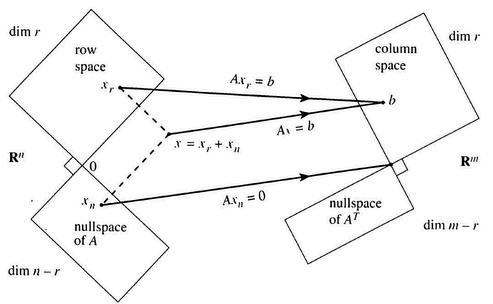
\includegraphics[scale=0.5]{./figs/10/10-1.png}
\end{figure}

我们观察到以下几点:
\begin{enumerate}
	\item 矩阵的行空间与解空间(零空间)互为正交补(直观理解两个空间就是互相垂直且互为补空间),这一点应当是在正交的内容中有所提及的;
	\item 矩阵的列空间与其转置矩阵的零空间互为正交补,这一点实际与上一条等价.
\end{enumerate}

接下来我们来看行秩(列秩比较显然,此处不再详细展开).我们首先得到解空间的维数,这可以直接
根据维数公式得到:$\dim N(A)=n-r(A)$,根据正交补的性质,我们的可以得到行秩即为
$n-(n-r(A))=r(A)$.于是我们得到了一个基于正交补的行秩解释.

\section{相抵标准形}
此处我们需要首先回顾一个基本定理:
\begin{theorem}
	初等变换不改变矩阵的秩(包括行变换和列变换).
\end{theorem}
由这一定理我们可以推导出相抵标准形:
\begin{theorem}
	若$r(A_{m \times n})=r$,则存在可逆矩阵$P$和$Q$,使得
	$$PAQ=\begin{pmatrix}
		E_r & 0 \\ 0 & 0
	\end{pmatrix}=U_r,$$
	其中$E_r$表示$r$阶单位矩阵.
\end{theorem}
这一定理证明直接使用定理4以及可逆矩阵可以拆分为初等矩阵的乘积即可.
其中$U_r$称为相抵标准形.我们称两个矩阵相抵即两个矩阵可以通过一系列
初等变换可以互相转化.由此我们得到关于矩阵相抵的两个等价命题:

1. 矩阵$A$与$B$相抵$\iff$存在可逆矩阵$P$和$Q$使得$PAQ=B$;

2. 矩阵$A$与$B$相抵$\iff r(A)=r(B)$.

\begin{example}
	设$A=\begin{pmatrix}
		1 & 0 & 2 & -4 \\ 2 & 1 & 3 & -6 \\ -1 & -1 & -1 & 2
	\end{pmatrix}$, 求

	\textup{(1)}$A$的秩$r$和相抵标准形;

	\textup{(2)}$3$阶可逆矩阵$P$和$4$阶可逆矩阵$Q$使得$PAQ=\begin{pmatrix}
		E_r & 0 \\ 0 & 0
	\end{pmatrix}$.
\end{example}

关于相抵标准形,我们需要在此补充一个常用的技术,即相抵标准形的分解:

我们对$s \times n$矩阵$\begin{pmatrix}
	E_r & O \\ O & O
\end{pmatrix}$有一种很重要的分解:
$$\begin{pmatrix}
	E_r & O \\ O & O
\end{pmatrix}=\begin{pmatrix}
	E_r \\ O
\end{pmatrix}\begin{pmatrix}
	E_r & O
\end{pmatrix}$$ 由此我们可以知道任意一个非零矩阵都可以被分解成一个列满秩矩阵和一个
行满秩矩阵的乘积:

$$A=P\begin{pmatrix}
	E_r & O \\ O & O
\end{pmatrix}Q=P\begin{pmatrix}
	E_r \\ O
\end{pmatrix}\begin{pmatrix}
	E_r & O
\end{pmatrix}Q$$
记$P_1=P\begin{pmatrix}
	E_r \\ O
\end{pmatrix}$,$Q_1=\begin{pmatrix}
	E_r & O
\end{pmatrix}Q$,则$A=P_1Q_1$,且$P_1$和$Q_1$分别为列满秩、行满秩矩阵.

我们可以利用相抵标准形解决很多问题,例如下一节中部分秩不等式的证明:
\begin{example}
	\textup{(1)}$r\begin{pmatrix}
		A & O \\ O & B
	\end{pmatrix}=r(A)+r(B)$.

	\textup{(2)}$r\begin{pmatrix}
		A & D \\ O & B
	\end{pmatrix}\ge r(A)+r(B)$,
	$r\begin{pmatrix}
		A & O \\ C & B
	\end{pmatrix}\ge r(A)+r(B)$.
\end{example}

\section{秩不等式}
本节的内容实际上部分内容有一定的技巧性,对于荣誉课程来说还是以理解为主(所以
其实本节中提到的很多内容都只是介绍性的,而非要求大家熟练掌握,但是遇见了要有
一些基本的思路而不能完全不理解),可能下面列出定理的时候显得比较繁冗,但是实
际上我们更重视其中的理解而非硬套结论.

我们首先给出一些常见的秩相关的不等式或等式,这些式子希望各位同学能够理解其含义,
而非机械记忆套用.下面这些等式/不等式的证明方式非常多,实际上可以利用之前所说化为
相抵标准形的方法,也可以利用线性相关性的方法,也可以回到线性映射进行考量.总之
解决的方法非常多,希望各位同学能熟练推导理解.
\begin{enumerate}
	\item $r(A)=r(PA)=r(AQ)=r(PAQ)$,其中$P$、$Q$可逆
	\item $|r(A)-r(B)|\le r(A\pm B) \le r(A)+r(B)$
	\item $r(AB) \le \min\{r(A),\ r(B)\}$
	\item $r(A)=r(A^\mathrm{T})=r(AA^\mathrm{T})=r(A^\mathrm{T}A)$(注意第二个等号需要实矩阵作为前提条件)
	\item $A \in \mathbf{F}^{s \times n}$,$B \in \mathbf{F}^{n \times m}$,
	则$r(AB) \ge r(A)+r(B)-n$.(可以视为结论6的推论,特例$AB=O$时有$r(A)+r(B)\le n$)
	\item $r(ABC) \ge r(AB)+r(BC)-r(B)$.(还可以考虑A,B,C相等的特殊情况的结果)
\end{enumerate}

分块矩阵的相关公式在上一小节的例题中已经书写过,此处不再重复.

一般而言,解决较为复杂的秩的问题时,我们可以采用如下方法:

(1)利用(分块)矩阵初等变换;

(2)利用线性方程组解的一般理论(将在专题五讲解);

(3)利用向量组线性相关性;

(4)利用已知的矩阵秩的等式和不等式.实际上等式很多时候基于可逆矩阵变换或者两个不等号夹逼.

相关方法的应用都在本节最后的习题中有所体现,当然首要的任务是掌握上述基本的秩不等式的证明,
很多也利用了上面的思想,并且解法不唯一.

\vspace{2ex} 
\centerline{\heiti \Large 内容总结}

\vspace{2ex} 

\centerline{\heiti \Large 习题}
\vspace{2ex} 
{\kaishu }
\begin{flushright}
    \kaishu

\end{flushright}
\centerline{\heiti A组}
\begin{enumerate}
	\item 
\end{enumerate}
\centerline{\heiti B组}
\begin{enumerate}
	\item 
\end{enumerate}
\centerline{\heiti C组}
\begin{enumerate}
	\item 
\end{enumerate}